\chapter{LE2ML: un \textit{workbench} modulaire pour l'apprentissage machine}
\label{chap:6}

\section{Introduction}

Grâce aux chapitres précédents, il a été montré que les \textit{wearable devices} sont de plus en plus utilisés dans le processus de reconnaissance d'activités au sein des habitats intelligents. Aussi, ces dispositifs ont également été employés dans l'objectif de répondre à plusieurs autres problématiques relatives à l'assistance des résidents de ces habitats, au sens large. Néanmoins, l'engouement croissant pour les \textit{wearable devices} a permis d'identifier plusieurs problématiques quant à leur utilisation dans ce contexte de recherche particulier. En effet, il a été évalué que la plupart des différentes architectures d'habitats intelligents qui ont été proposées n'ont pas été conçues dans une optique évolutive. Ainsi, celles-ci ne permettent pas d'y intégrer de manière rapide et efficace de nouveaux capteurs, comme les \textit{wearable devices}, ou de nouveaux composants logiciels pour effectuer le processus de reconnaissance d'activités et l'assistance aux résidents.

Pour ce travail, l'intégration des \textit{wearable devices} dans les architectures de maisons intelligentes s'est concentrée avant tout sur l'aspect logiciel plutôt que matériel pour les méthodes de reconnaissances que ces dispositifs proposent. En effet, tout comme pour la reconnaissance d'activités réalisée de manière classique, c'est-à-dire, en exploitant les capteurs et effecteurs statiques présents dans l'habitat, les différents processus proposés par les dispositifs sont, dans une vaste majorité des cas, encapsulés au sein d'un unique composant logiciel immuable. De la même manière, la réutilisation de mécanismes communs, le déploiement de ces méthodes et leur modification demeurent alors des tâches complexes à mettre en \oe{}uvre.

Malgré cela, certains travaux ont fait mention de l'emploi d'un \textit{workbench} d'apprentissage machine afin de traiter les données produites par les \textit{wearable devices} et de réaliser la reconnaissance d'activité \citep{Chapron2018}. D'un point de vue académique, ces outils ne sont pas nouveaux et ils permettent un prototypage rapide, la visualisation des données ainsi qu'une meilleure reproductibilité des méthodes expérimentales et une meilleure réutilisation des composants logiciels \citep{Holmes1994,Langlois2008}. À titre d'exemple, l'outil le plus connu et le plus répandu dans la littérature est \acs{WEKA}. Il s'agit d'un \textit{workbench} open source issue de la recherche académique qui supporte un grand nombre d'algorithmes d'apprentissage machine supervisés et non supervisés \citep{Witten2016}. Celui-ci a été utilisé en tant que librairie dans la méthode de reconnaissance des types de sols présentée au chapitre \ref{chap:4}. Néanmoins, bien que ce \textit{workbench} offre un large éventail d'options, son utilisation reste relativement gourmande en termes d'utilisation des ressources de calcul et de mémoire. De plus, les fonctionnalités offertes par cet outil demeurent particulièrement contraignantes à étendre et, en raison de sa conception, il n'est pas particulièrement adapté pour être utilisé dans l'architecture d'habitats intelligents distribuée qui a été introduite dans le chapitre précédent. Par ailleurs, avec la tendance qui entoure actuellement l'intelligence artificielle, ce type d'outil devient de plus en plus populaire depuis que des fournisseurs de \textit{cloud} publics, tels qu'\textit{Amazon AWS}, \textit{Google Cloud Plateform} et \textit{Microsoft Azure} ont introduit des versions grand public de ces applications. Comme elles font partie de la vaste liste de services payants proposés par chaque fournisseur, les \textit{workbench} d'apprentissage machine peuvent bénéficier de l'évolutivité qu'offre le \textit{cloud}. Cependant, comme ils sont considérés comme des services d'usage général, les mécanismes internes des techniques d'apprentissage machine ont été complètement occultés afin de les rendre accessibles à tous.

Ainsi, ce dernier travail présente \acs{LE2ML} (\acl{LE2ML}), un nouveau type de \textit{workbench} pour l'apprentissage machine qui repose sur l'utilisation de microservices. De la même manière que pour l'implémentation de l'architecture proposée, cette conception logicielle a été choisie, car la technologie des microservices permet une meilleure évolutivité, des déploiements plus sûrs et plus rapides ainsi qu'une meilleure isolation des pannes \citep{Dragoni2017}. Cependant, l'avantage principal d'une telle conception concerne l'aspect modulaire que permettent les microservices. Ainsi, ce \textit{workbench} demeure un outil agnostique tant en termes de langages de programmation que de plateformes supportées qui peut être déployé dans n'importe quel environnement, et ce, sans aucune contrainte complexe.

La suite de ce chapitre comporte une première section qui propose un état de l'art en matière de \textit{workbench} pour l'apprentissage machine, car ceux-ci ont joué, depuis plusieurs années, un rôle important dans différents champs de recherche. Ensuite, la section suivante introduit \acs{LE2ML}, le \textit{workbench} proposé et une expérimentation pour évaluer son fonctionnement et valider les résultats attendus est décrite dans une troisième section. Finalement, dans une dernière partie, ce chapitre dresse une conclusion quant à ce dernier travail.

\section{État de l'art}

Selon \cite{Langlois2008}, un \textit{workbench} d'apprentissage machine est un outil qui fourni une interface unifiée qui permet d'exploiter un certain nombre d'algorithmes d'apprentissage dans le but de traiter différents problèmes que ces méthodes peuvent potentiellement résoudre. Ainsi, au cours des dernières années, plusieurs de ces outils ont été développés et exploités dans divers domaines de recherche tels que la bio-informatique \citep{Larranaga2006}, la cybersécurité \citep{Handa2019}, la santé \citep{Rajkomar2019}, et plus particulièrement pour la reconnaissance d'activité à l'intérieur des habitats intelligents \citep{Ramirez-Prado2019}. Cette section décrit donc trois de ces outils d'apprentissage machine open-source qui sont parmi les plus utilisés dans la littérature. Ceci dans l'objectif principal d'identifier le besoin qui a motivé l'introduction de \acs{LE2ML}.

\subsection{WEKA}

\acs{WEKA} constitue un ensemble d'algorithmes d'apprentissage machine développé en Java qui a été introduit en 1994 principalement pour faciliter les tâches de forage de données (\textit{data mining}) \citep{Holmes1994}. Plus précisément, cet outil contient plusieurs fonctionnalités qui permettent d'effectuer du prétraitement de données, de la classification, de la régression, du \textit{clustering}, des règles d'association, de l'apprentissage profond et de la visualisation. Bien que \acs{WEKA} suggère son propre format de fichier natif (\acl{ARFF} ou \acs{ARFF}), il supporte également les fichiers \acs{CSV}, les fichiers Matlab ainsi que la connectivité à plusieurs bases de données \textit{via} \ac{JDBC}. En ce qui concerne le prétraitement des données, \acs{WEKA} propose un grand nombre de méthodes allant de la simple suppression d'attributs pour les ensembles de données à des opérations avancées comme l'analyse par composantes principales (\acs{PCA}).

Dans sa première version, \acs{WEKA} était uniquement exploitable au travers d'une interface en ligne de commande (\acs{CLI}). Aujourd'hui, bien qu'il soit toujours possible d'utiliser la \acs{CLI}, cet outil offre la possibilité d'être inclus en tant que dépendance d'un projet Java ou \textsf{R} \citep{Hornik2009}. De plus, il peut surtout être utilisé à travers plusieurs types d'interfaces graphiques. Dans un premier temps, la première possibilité demeure l'\emph{explorer}, où l'utilisateur peut mettre en place rapidement des techniques de manipulation des données (filtrage, classification, \textit{clustering} et visualisation), sans avoir besoin d'écrire de code. Dans un second temps, \acs{WEKA} propose une interface propre aux expérimentations : l'\emph{experimenter}. Il s'agit d'un outil permettant d'exécuter en parallèle, c'est-à-dire, selon différents processus sur une même machine ou sur différents ordinateurs d'un réseau, plusieurs expériences d'apprentissage machine afin d'évaluer les méthodes de classification et de régression. La troisième interface proposée par \acs{WEKA}, appelée \emph{knowledge flow}, offre la possibilité de réaliser les mêmes tâches qu'avec l'interface \emph{explorer}. Néanmoins, celles-ci sont représentées sous forme de blocs qui doivent être manipulés pour construire un processus de flux opérationnel (\textit{workflow}) comme le montre la figure \ref{fig:weka}. Cette dernière illustre un exemple d'utilisation de l'interface \emph{knowledge flow} pour un processus de classification sur les données du jeu de données iris \citep{Asuncion2007}. Dans cet exemple, l'algorithme \acs{KNN}, configuré avec $k=1$ voisin a été utilisé et la performance de la classification a été évaluée selon la technique de la séparation en $80/20$, c'est-à-dire, $80\%$ des données sont utilisées pour la phase d'entrainement, tandis que les $20\%$ restants sont exploités lors de la phase de reconnaissance.

\begin{figure}[H]
	\centering
	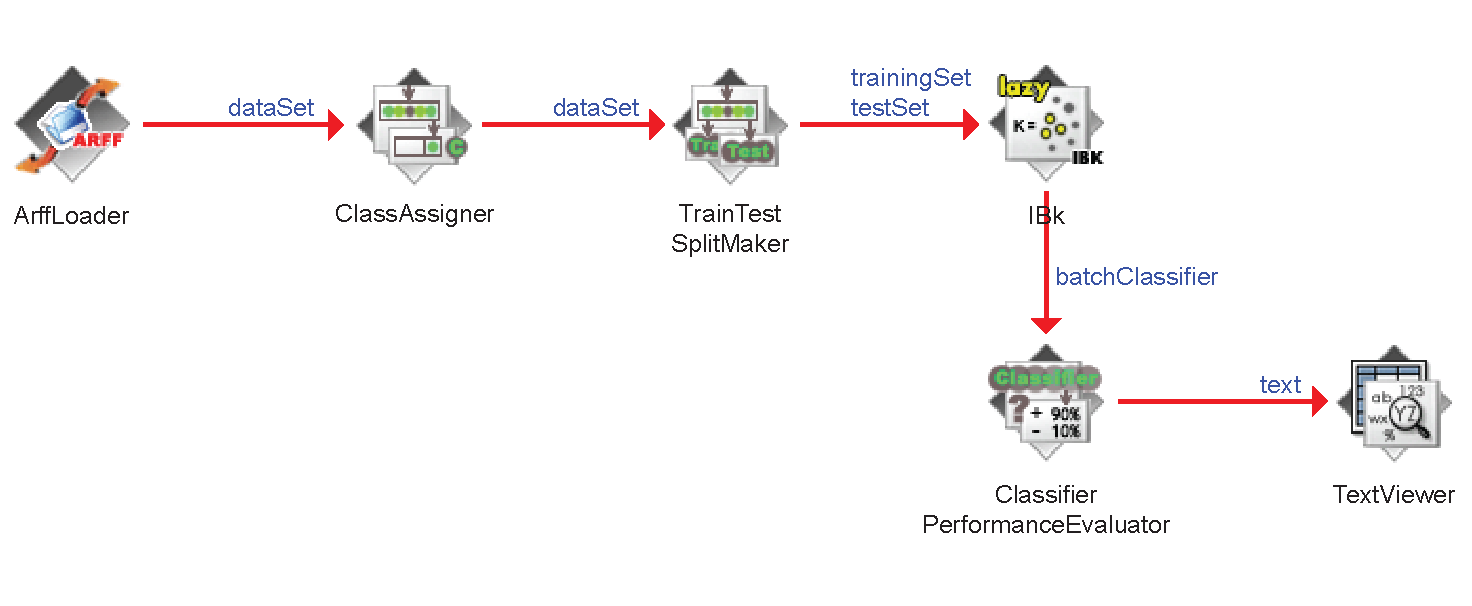
\includegraphics[width=.9\linewidth]{chapter6/weka.pdf}
        \caption{Exemple de l'interface \textit{knowledge flow} de \acs{WEKA} qui décrit un processus de classification sur le jeu de données iris avec l'algorithme \acs{KNN} où $k=1$ voisin et évaluée selon la technique de la séparation $80/20$.}
	\label{fig:weka}
\end{figure}

\acs{WEKA} est probablement le \textit{workbench} d'apprentissage machine le plus connu et le plus utilisé puisqu'il s'agit d'un outil portable \citep{Bouckaert2010} offrant un large éventail de possibilités pour réaliser facilement des processus liés à l'apprentissage machine. Cependant, cet outil présente plusieurs inconvénients. Premièrement, comme il est écrit en Java et qu'il repose sur une ancienne base de code, sa capacité à traiter une grande quantité de données et la rapidité des différentes opérations sont profondément affectées par une consommation importante de ressources. Plus récemment, un gestionnaire de paquets a été introduit afin de permettre à des développeurs tiers d'étendre les fonctionnalités de base du \textit{workbench} \citep{Hall2009}. Néanmoins, bien que ces nouvelles fonctionnalités ont permis à \acs{WEKA} de devenir plus flexible, le développement de ces paquets n'est possible qu'en Java et ceux-ci doivent respecter les contraintes d'intégration dans l'outil.

\subsection{RapidMiner}

RapidMiner, également connu sous le nom de \acs{YALE} (\acl{YALE}) \citep{Ritthoo2003,Hofmann2014}, a été développé à partir de 2001 puis rebaptisé en RapidMiner en 2007.  De la même manière que \acs{WEKA}, RapidMiner propose un environnement qui repose sur du code Java pour mettre en \oe{}uvre des techniques d'apprentissage machine. Cependant, contrairement à \acs{WEKA}, cet outil n'offre qu'une seule interface qui permet de définir des flux opérationnels à la façon de l'interface \textit{knowledge flow}. En effet, ces processus sont décrits à partir de blocs élémentaires appelés opérateurs. Il est alors possible pour l'utilisateur de composer une chaîne d'opérateurs en plaçant ces blocs sur un canevas et en câblant leurs ports d'entrée et de sortie, comme le montre la figure \ref{fig:rapid_miner}. Bien que \acs{WEKA} soit intégré dans RapidMiner en tant que dépendance utilisée pour plusieurs blocs, la majorité d'entre eux permettent d'étendre nombreux aspects de l'apprentissage machine qui ne sont pas nécessairement couverts par \acs{WEKA}.

Par ailleurs, RapidMiner inclut également la possibilité d'ajouter des paquets développés par des tiers afin d'améliorer ses capacités initiales. De plus, il permet l'utilisation d'un bloc de script où il est possible d'écrire du code en syntaxe Java ou Groovy. En ce sens, RapidMiner apparait tout aussi flexible que \acs{WEKA}. Cependant, puisqu'il repose sur une conception logicielle comparable et un langage de programmation de base identique, ce \textit{workbench} souffre des mêmes inconvénients. En outre, il est possible de dire que RapidMiner ne convient pas au déploiement d'applications expérimentales dans un contexte de recherche, car il ne dispose pas d'interface en ligne de commande et il n'est pas possible de l'utiliser comme une librairie dans une application.

\begin{figure}[H]
	\centering
	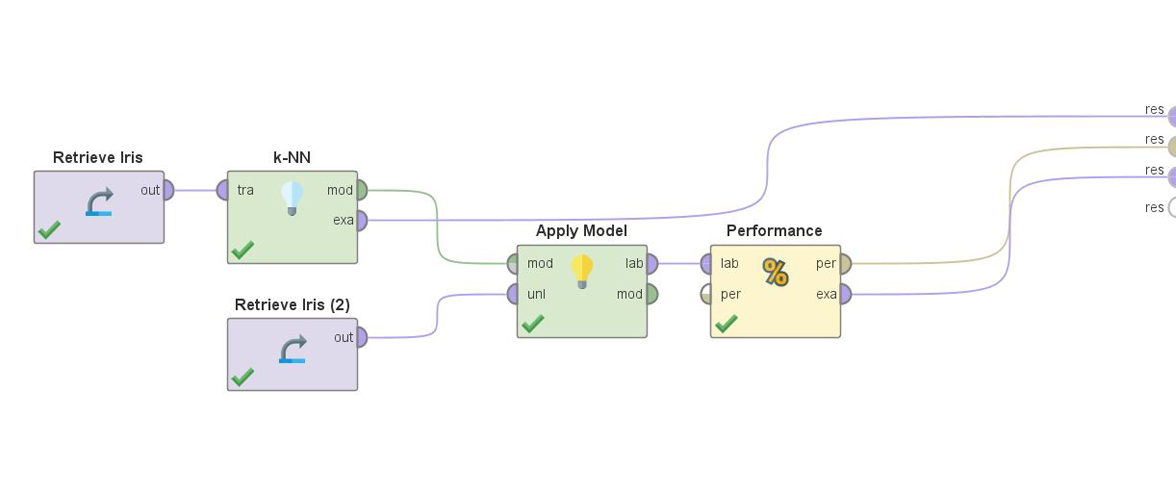
\includegraphics[width=.9\linewidth]{chapter6/rapid_miner.jpg}
        \caption{Exemple de chaîne d'opérateurs dans l'outil RapidMiner qui décrit un processus de classification sur le jeu de données iris avec l'algorithme \acs{KNN} où $k=1$ voisin et évaluée selon la technique de la séparation $80/20$.}
	\label{fig:rapid_miner}
\end{figure}

\subsection{Orange}

Orange est le dernier \textit{workbench} d'apprentissage machine, parmi les plus mentionnés dans la littérature, qui est présenté dans ce chapitre. Introduit en 1997, les fonctionnalités de base de cet outil ont été initialement conçues en \verb!C++! et sa couche logicielle supérieure (c'est-à-dire les modules et l'interface graphique) était développée en Python \citep{Demsar2004,Demsar2013}. Cependant, depuis 2015, Orange a été entièrement redéveloppé. L'ancien noyau \verb!C++! a été remplacé entièrement par du code Python et l'interface graphique a également été revue. De la même manière que \acs{WEKA}, Orange offre la possibilité soit d'être importé en tant que librairie dans un script Python, soit d'être utilisé comme outil à part entière grâce à interface graphique également basée sur l'utilisation de composants. En effet, comme le montre la figure \ref{fig:orange}, Orange permet également de manipuler des \emph{widgets} disposés sur un canevas qui, une fois reliés entre eux, permettent de définir un \emph{schéma} qui représente le flux opérationnel du processus d'apprentissage machine à réaliser. En outre, ce \textit{workbench} offre également la possibilité d'importer des \emph{widgets} personnalisés par l'intermédiaire d'un gestionnaire de paquets.

\begin{figure}[H]
	\centering
	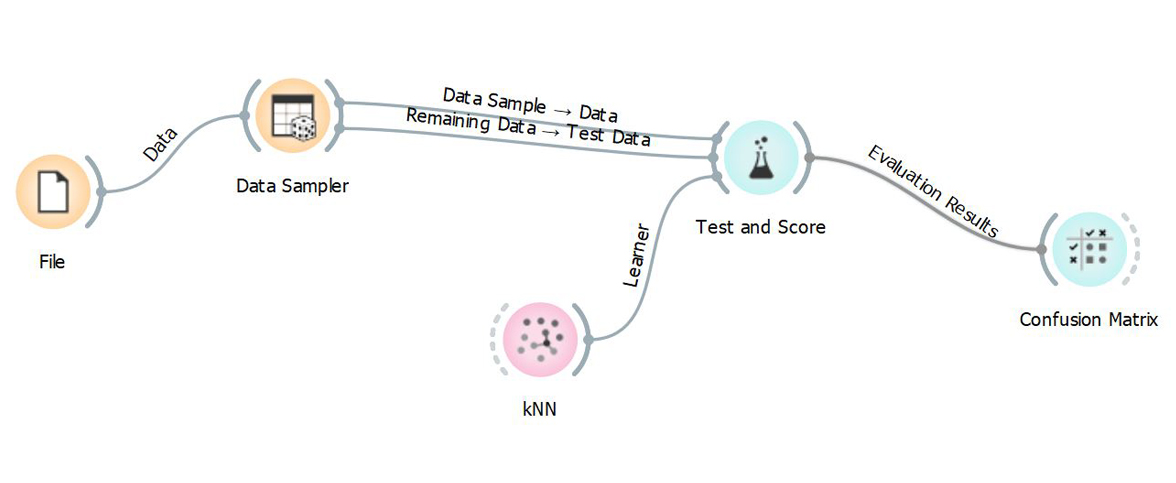
\includegraphics[width=.9\linewidth]{chapter6/orange.jpg}
        \caption{Exemple d'un \emph{schéma} dans Orange qui décrit un processus de classification sur le jeu de données iris avec l'algorithme \acs{KNN} où $k=1$ voisin et évaluée selon la technique de la séparation $80/20$.}
	\label{fig:orange}
\end{figure}

De la même manière que WEKA, puisqu'une intégration dans un programme Python est possible, Orange semble être tout autant susceptible d'être employé dans la conception d'applications académiques. De plus, étant donné que la version la plus récente d'Orange (Orange3) repose sur plusieurs outils modernes tels que NumPy\footnote{\url{https://numpy.org}}, SciPy\footnote{\url{https://www.scipy.org}} et scikit-learn\footnote{\url{https://scikit-learn.org}}, les possibilités de créer des widgets personnalisés sont illimitées. Par ailleurs, l'exécution d'un processus de classification réalisé avec Orange a montré une consommation de ressources (temps calcul et utilisation mémoire) plus raisonnable que pour le même processus effectué avec \acs{WEKA}. En revanche, les recommandations fournies qui documentent la conception de widgets personnalisés ne sont pas triviales et se limitent à du code Python.

\section{Solution proposée}

Dans la section précédente, les trois principaux \textit{workbench} d'apprentissage machine ont été présentés dans le but de déterminer les problématiques de chacune de ces solutions. Ainsi, il est apparu que tous ces outils présentent le même principal inconvénient, c'est-à-dire, une forte dépendance à leur contexte d'utilisation. En effet, toutes permettent d'intégrer des composants logiciels personnalisés, néanmoins ceux-ci doivent être conçus pour répondre aux exigences de l'outil pour lequel ils sont développés. De plus, dans un contexte de recherche académique, ces paquets additionnels peuvent devenir difficiles à maintenir. En effet, ils doivent être installés manuellement sur chacun des dispositifs qui composent l'environnement (\textit{p. ex.} ordinateurs ou serveurs), ce qui provoque indubitablement des problèmes de déploiement et de réutilisation.

Ainsi, ce chapitre présente \acs{LE2ML}\footnote{\url{https://github.com/FlorentinTh/LE2ML}} (\acl{LE2ML}), un nouveau type de \textit{workbench} d'apprentissage machine qui, comme pour l'architecture introduite précédemment, s'appuie sur la technologie des microservices. Bien que cet atelier ait été spécifiquement conçu pour être utilisé dans notre architecture, il est parfaitement possible de le faire fonctionner dans des environnements plus traditionnels tels qu'un serveur dans une architecture de maison intelligente monolithique ou un simple ordinateur. La seule contrainte préalable est d'y installer le moteur de conteneurs Docker. LE2ML a été développé dans le but d'être modulaire. De ce fait, le composant principal de la conception de son architecture logicielle demeure une \acs{API} (\acl{API}) \acs{REST}. Cette API est principalement chargée de piloter tous les autres composants logiciels du \textit{workbench} qui sont considérés comme des modules que n'importe qui peut développer et intégrer fonctionnalités de base selon les besoins. Enfin, une application web a également été développée pour faciliter les interactions avec l'\acs{API}. La figure \ref{fig:containers_workbench} présente un exemple de déploiement possible pour \acs{LE2ML}. En effet, celle-ci illustre l'organisation des conteneurs et de leurs réseaux superposés qui sont nécessaires pour que le \textit{workbench} fonctionne sur notre architecture. Ainsi, cette figure va guider les explications données dans le reste de ce chapitre.

\begin{figure}[H]
	\centering
	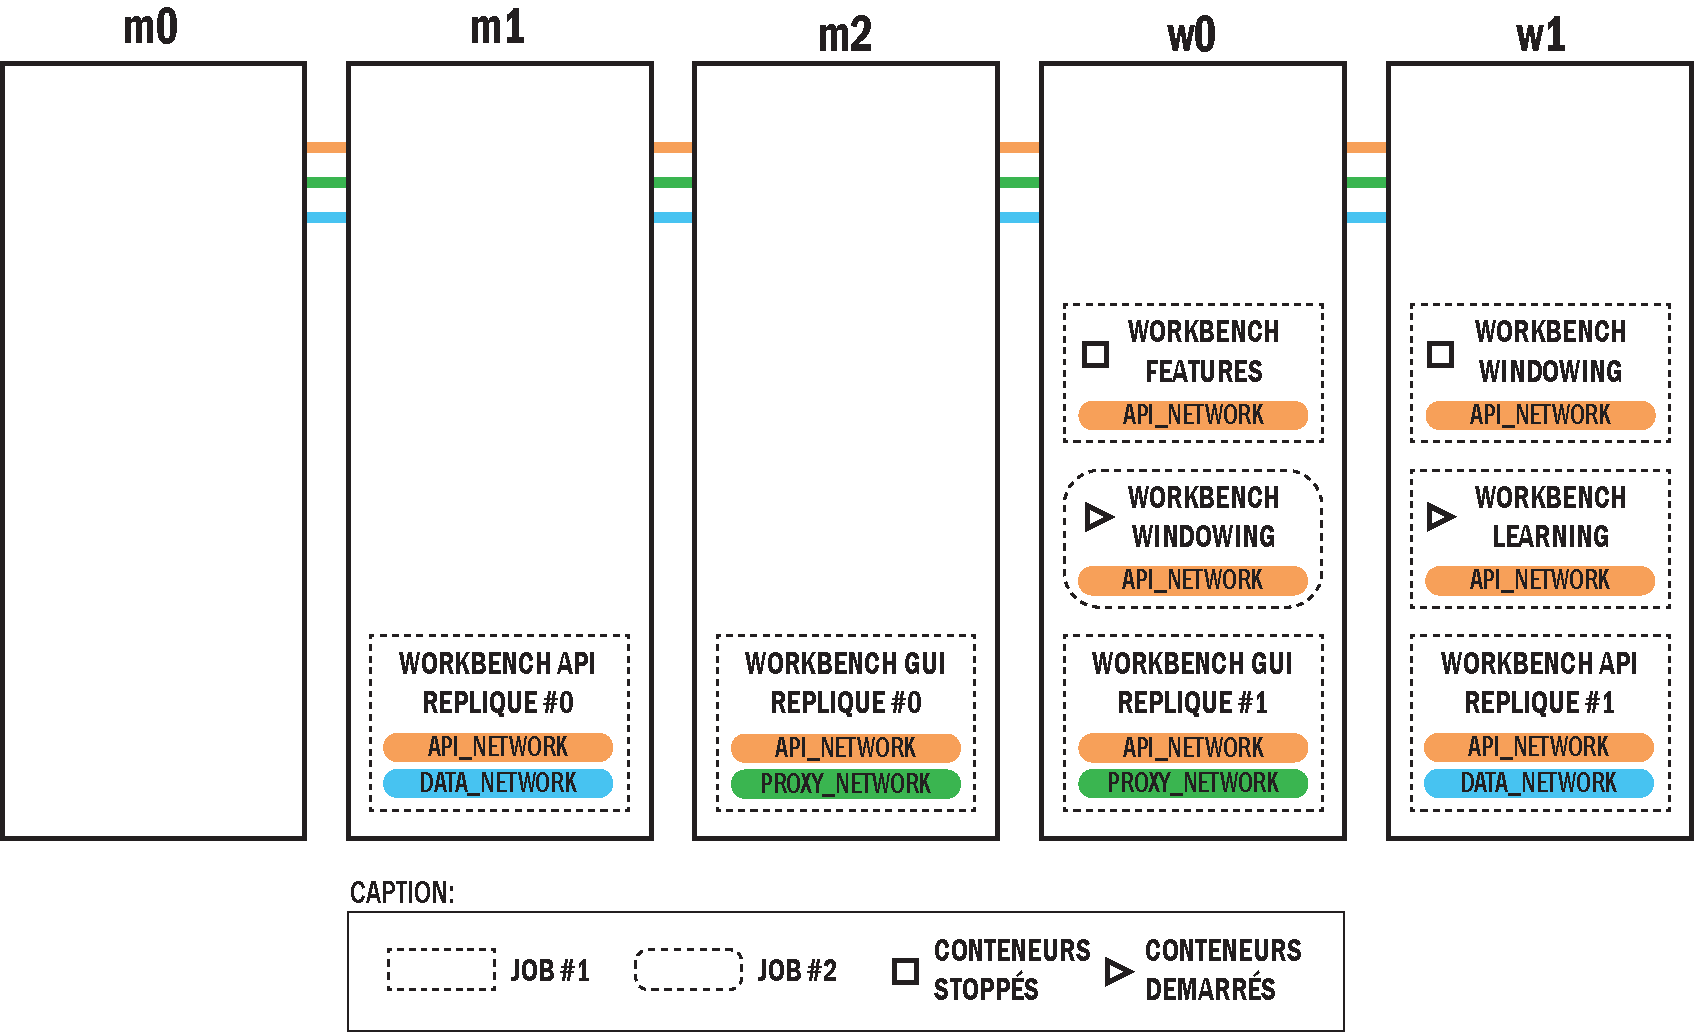
\includegraphics[width=.9\linewidth]{chapter6/containers_workbench.pdf}
        \caption{Exemple de placement des conteneurs et leurs réseaux superposés sur chaque n\oe{}ud de l'architecture proposée précédemment lors du déploiement de \acs{LE2ML}.}
	\label{fig:containers_workbench}
\end{figure}

\subsection{\acs{API} \acs{REST}}

En tant que composant logiciel principal dans la conception de \acs{LE2ML}, l'\acs{API}, a été développée en JavaScript grâce à Node.js\footnote{\url{https://nodejs.org}}. Cet outil constitue un environnement d'exécution basée sur le moteur V8\footnote{\url{https://v8.dev}} qui permet de créer des applications côté serveur en JavaScript. Ensuite, le \textit{framework} Express.js\footnote{\url{https://expressjs.com}} a également été employé pour la création de l'\acs{API} \acs{REST}. Plus précisément, celui-ci a permis de simplifier la définition des fonctions de traitement associées à des requêtes \acs{HTTP} répondant aux différentes \acs{URI} de l'application (cf. section \ref{sec:services_web}).

Par ailleurs, comme le montre la figure \ref{fig:containers_workbench}, le service qui contient l'\acs{API} a été déployé en tant que service utilisant deux répliques qui peut être exécuté soit sur des n\oe{}uds de type \textit{manager} ou \textit{worker}. Ce déploiement demeure la recommandation suggérée puisque, dans un tel cas, l'accessibilité de l'\acs{API} est garantie, même en cas de défaillance d'un n\oe{}ud de l'architecture. Toutefois, en fonction de la demande en ressource, c'est-à-dire, lorsque l'API doit traiter un grand nombre de requêtes, il est possible de procéder à une mise à l'échelle du service afin d'éviter un ralentissement de l'ensemble du \textit{workbench}. De plus, bien que le service de l'\acs{API} fournit son propre réseau superposé (\texttt{api\_network}), ce service, incluant ses répliques, doit être relié au réseau de données (\texttt{data\_network}) afin de pouvoir communiquer avec la base de données déployée au sein de l'architecture. En effet, l'\acs{API} doit être en mesure de manipuler les données principalement relatives aux utilisateurs, tâches, sources de données et algorithmes d'apprentissage machine, de fenêtrage et d'extraction de caractéristiques qui sont utilisés dans les modules de \acs{LE2ML}. Cette implémentation a été préférée dans le cadre d'une utilisation avec l'architecture présentée dans le chapitre précédent. Cependant, la mise à disposition d'une base de données non relationnelle n'est pas une contrainte imposée pour assurer le fonctionnement du \textit{workbench} dans des environnements différents.

L'objectif principal de l'\acs{API} de \acs{LE2ML} est d'exécuter plusieurs processus (\emph{jobs}) d'apprentissage machine simultanés grâce à la définition de \textit{pipelines} pour ce processus. Pour ce faire, l'API est chargée d'orchestrer le démarrage des différents modules du \textit{workbench} qui s'exécutent alors à l'intérieur de conteneurs. Lorsque tous les modules ont terminé, le \textit{pipeline} d'apprentissage machine est complété et la performance de la reconnaissance est donnée selon plusieurs métriques d'évaluation. De plus, l'\acs{API} propose également plusieurs fonctionnalités de base qui ne sont pas des modules, car elles sont complémentaires au processus d'apprentissage machine. Celles-ci comprennent l'importation de fichiers de données, la gestion de ces fichiers importés ou nouvellement créés, la visualisation des données, la gestion de l'authentification et des autorisations pour les utilisateurs et les applications, la gestion des utilisateurs et de leur rôle ainsi que la gestion des modules.

La définition d'un \textit{pipeline} d'apprentissage machine se fait par le biais d'un fichier \ac{YAML}. Cette approche a été choisie, car un tel type de fichier demeure plus facile à lire et à écrire que le format \acs{JSON}. Par ailleurs, le \acs{YAML} est un format qui se prête particulièrement bien avec l'utilisation de systèmes de gestion de versions (\aclp{VCS} ou \acsp{VCS}) pour être partagés entre plusieurs expérimentateurs au sein d'une équipe de recherche. Une fois transmis à l'\acs{API}, le fichier de définition du \textit{pipeline} est converti en format JSON afin d'être validé grâce à un schéma, puis il est stocké sur le système de fichiers distribué. Ensuite, le contenu du fichier est analysé par l'\acs{API} afin que toutes les tâches qui composent le \textit{pipeline} soient lancées de manière consécutive. Un exemple d'un tel fichier de définition est présenté en figure \ref{fig:pipeline_conf}.

\begin{figure}[H]
	\centering
	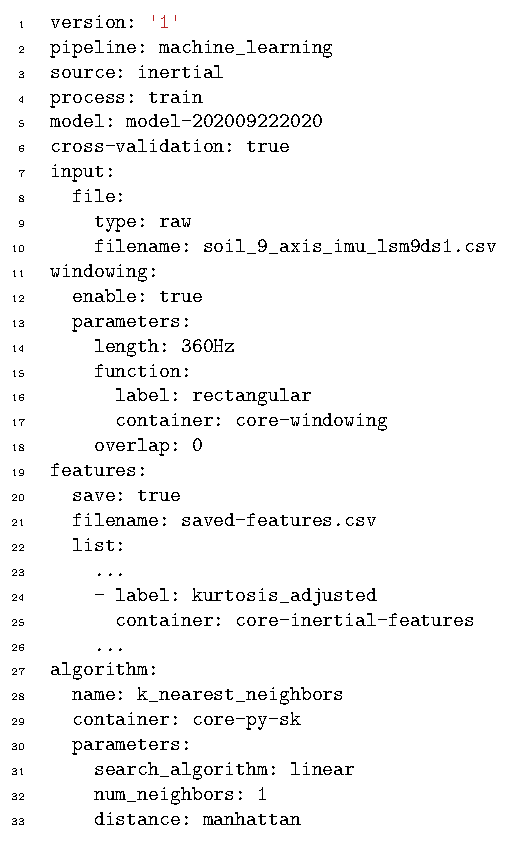
\includegraphics[width=.5\linewidth,keepaspectratio]{chapter6/pipeline_conf.pdf}
        \caption{Exemple d'un fichier de définition d'un \textit{pipeline} qui décrit la phase d'entrainement d'un processus d'apprentissage machine traditionnel.}
	\label{fig:pipeline_conf}
\end{figure}

Dans un premier temps, l'utilisateur doit préciser le type de \textit{pipeline} qui doit être réalisé. Les possibilités sont soit apprentissage machine \texttt{machine\_learning}, soit apprentissage profond (\texttt{deep\_learning}). Une autre propriété obligatoire concerne la source de données, ce qui correspond au type de données qui sont traitées au cours le processus (\textit{p. ex.} des données inertielles ou vocales). Par ailleurs, lorsqu'il s'agit d'un \textit{pipeline} définissant un processus d'apprentissage machine traditionnel, la propriété \texttt{process} doit également être déclarée. Les valeurs possibles sont \texttt{train} et \texttt{test} qui font respectivement référence aux phases d'entrainement de prédiction pour un tel processus. Il est également possible d'y attribuer la valeur \texttt{none}. Ceci dans le but de permettre aux utilisateurs de réaliser uniquement certaines tâches qui précèdent le processus d'apprentissage, comme l'extraction de caractéristiques. Comme montré par cet exemple, dans le cas où le pipeline doit compléter la phase d'entrainement, l'attribut \texttt{model} doit aussi être fourni. Ainsi, le modèle de données qui a été entrainé par l'algorithme d'apprentissage soit sauvegardé sur le système de fichier pour être réutilisé ultérieurement (\textit{p. ex.} lors de la définition d'une phase de prédiction). De plus, la propriété \texttt{cross-validation} est la dernière propriété imposée lorsqu'il s'agit d'une phase d'entrainement. Elle permet de produire une estimation des performances de reconnaissance en évaluant le modèle nouvellement créé grâce à la méthode de la validation croisée en 10-plis. Ensuite, il est nécessaire de déclarer les données d'entrée sur lesquelles est appliqué le processus d'apprentissage machine. Actuellement, seules deux options sont autorisées, à savoir, la définition d'un fichier ou une connexion WebSocket. Lorsqu'il s'agit d'une source d'entrée de type WebSocket, l'\acs{URL} du serveur doit être indiquée. Sinon, les fichiers doivent être référencés selon leur nom et le type de données qu'ils contiennent (\textit{p. ex.} données brutes : \texttt{raw}). Enfin, le reste du contenu du fichier permet de décrire les différentes tâches et leurs paramètres associés qui sont utilisés lors de l'exécution des modules.

Pour compléter l'exécution des \emph{jobs}, l'\acs{API} a la responsabilité de démarrer les conteneurs selon la définition des tâches fournie dans les fichiers de définition des \textit{pipelines}. Ainsi, puisque certains conteneurs dépendent du résultat de la tâche précédente, ils sont lancés, pour un \emph{job} donné, les uns après les autres. Néanmoins, lorsqu'une même tâche est définie pour utiliser plusieurs conteneurs distincts, ceux-ci sont démarrés en même temps. Ils s'exécutent alors en parallèle. Enfin, les \emph{jobs} qui sont créés par les différents utilisateurs du \textit{workbench} sont également exécutés en parallèle, puisqu'ils sont indépendants les uns des autres quand bien même ils utilisent des images de conteneurs identiques. À titre d'exemple, la figure \ref{fig:containers_workbench} montre deux \emph{jobs} démarrées à des moments différents, mais dont le traitement est concurrent. En effet, il est possible d'observer que pour le premier \emph{job}, les tâches de fenêtrage et d'extraction de caractéristiques sont toutes les deux terminées alors que le conteneur d'apprentissage est toujours en cours d'exécution. À l'inverse, la tâche de fenêtrage pour le second \emph{job} vient juste de commencer et les autres conteneurs ne sont pas visibles, car ils n'ont pas encore été démarrés.

Pour qu'un conteneur devienne un module de \acs{LE2ML}, trois variables d'environnement doivent être définies, lors de son lancement. Il s'agit de l'identifiant unique du \emph{travail}, de l'identifiant unique de l'utilisateur ainsi que d'un jeton unique généré aléatoirement pour chaque conteneur. Le jeton est utilisé pour permettre à l'\acs{API} de faire le lien entre un conteneur en particulier et la tâche à laquelle il est rattaché. Par conséquent, il est possible de mettre à jour l'entrée du \emph{job} associé dans la base de données. En effet, une fois son traitement terminé, un module LE2ML doit communiquer son état (succès ou échec) à l'\acs{API} par le biais d'un \textit{endpoint} prévu à cet effet. De telles requêtes ne sont permises que si les conteneurs y sont autorisés. Cette vérification est établie grâce à une clé d'application générée au préalable pour chaque application.

Finalement, comme l'exécution des processus d'apprentissage machine implique la création de fichiers, les informations résultantes de chaque tâche du \textit{pipeline} qui doivent être écrites sur le système de fichiers sont isolées dans des dossiers séparés par \emph{job}. En ce sens, ces dossiers sont montés en tant qu'espaces de travail pour tous les conteneurs qui sont définis pour un \emph{job} donné.

\subsection{Application Web}

Pour faciliter l'interaction avec l'\acs{API}, nous avons jugé approprié de proposer une interface. De ce fait, une interface graphique\footnote{\url{https://github.com/FlorentinTh/LE2ML-GUI}} a été préférée à une interface de type \acs{CLI} (dont le développement n'est pas exclu dans un avenir proche). En effet, puisque les équipes de recherche sont, la plupart du temps, multidisciplinaires, la conception d'une \acs{GUI} a été priorisée, car ce type d'interface est plus simple à apprendre et à utiliser pour les utilisateurs néophytes. Cette application web a été développée grâce à des technologies modernes et sa conception repose principalement sur un \textit{framework} JavaScript développé spécifiquement qui supporte ECMAScript 6 et les versions supérieures de ce standard (ES6+). La stratégie de déploiement qui a été adoptée, pour ce composant applicatif s'exécute sur l'architecture proposée, reste la même que pour l'\acs{API}, c'est-à-dire, un service répliqué admettant deux instances qui peuvent être placées soit sur un n\oe{}ud \textit{manager}, soit sur un \textit{worker}.

La figure \ref{fig:le2ml_gui} montre une capture d'écran de la vue principale de l'interface qui permet de créer des \textit{jobs} d'apprentissage machine. Le fil d'Ariane (\texttt{A}) permet d'indiquer aux utilisateurs les étapes qui doivent être complétées pour définir toutes les tâches du \textit{pipeline}. Dans une vue précédente à cette capture d'écran, l'utilisateur doit sélectionner le type d'apprentissage machine qu'il souhaite réaliser (dans le cas présent, il s'agit d'un apprentissage machine traditionnel). Pour chaque étape du \textit{pipeline}, un ensemble de composants web (\texttt{B}) est proposé pour permettre aux utilisateurs de configurer chaque tâche de manière pratique. Cependant, bien qu'il soit possible de construire les fichiers de définition en interagissant avec l'interface graphique, une fonction d'import (\texttt{C}) a également été prévue pour permettre la réutilisation des définitions de \textit{pipeline} existantes. Dans ce contexte, les composants web pour chacune des étapes sont préremplis en fonction du contenu du fichier téléchargé.

Par ailleurs, cette interface offre également aux utilisateurs un moyen d'interagir avec toutes les autres fonctionnalités de l'\acs{API}. Le menu ``\textit{Data}'' (\texttt{d}) regroupe toutes les fonctionnalités liées aux fichiers de données d'entrée. Celles-ci comprennent un composant pour téléverser des fichiers, un gestionnaire de fichiers qui permet de naviguer dans les fichiers hébergés sur le système distribué, un outil de visualisation des données ainsi qu'un accès aux modules de prétraitement et de fusion des données. Le menu ``\textit{Jobs}'' (\texttt{e}) présente la liste des \textit{jobs} d'apprentissage machine en cours de traitement et terminés qui ont été créés par l'utilisateur connecté. Cette liste est mise à jour en temps réel grâce à la technologie \ac{SSE} qui permet à l'\acs{API} d'envoyer des notifications \textit{push} à l'application web. Par le biais de cette vue, il est également possible de télécharger les fichiers résultant d'un \textit{job} complété. Ces fichiers peuvent être soit un rapport comprenant des mesures d'évaluation de la performance pertinentes calculées pendant la phase d'entraînement, soit la liste des prédictions déterminées

\begin{figure}[H]
	\centering
	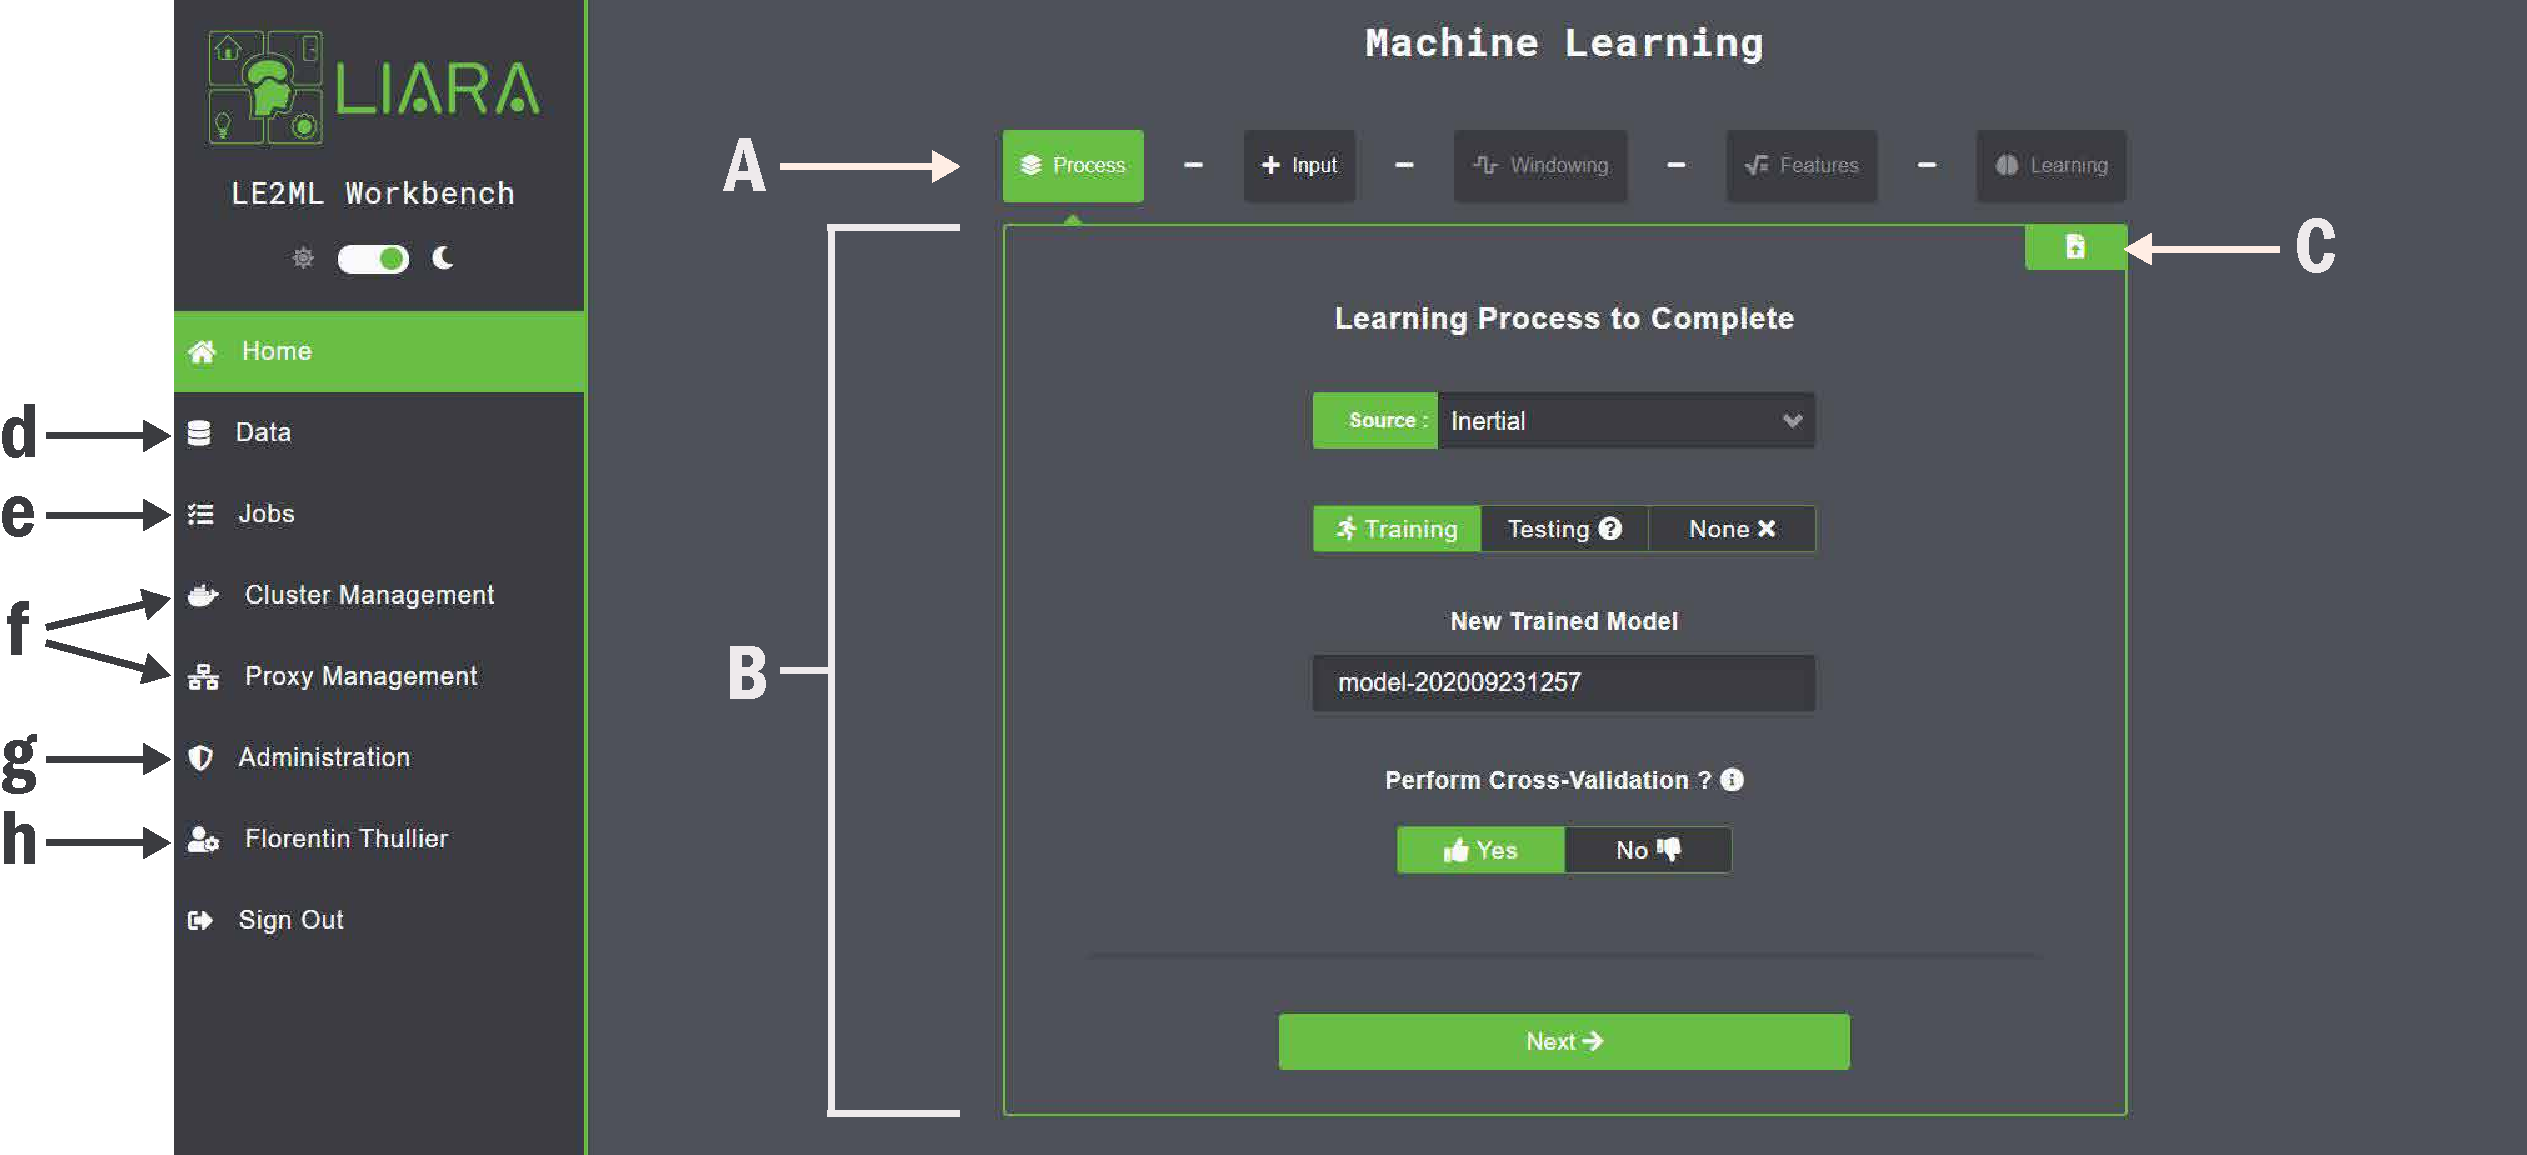
\includegraphics[angle=90,origin=c,height=.85\textwidth,keepaspectratio]{chapter6/le2ml_gui.pdf}
        \caption{Capture d'écran de l'application web qui montre la première étape de la définition d'un \textit{pipeline} d'apprentissage machine.}
	\label{fig:le2ml_gui}
\end{figure}

\noindent lors de la phase de test. Ensuite, les menus ``\textit{Cluster Management}'' et ``\textit{Proxy Management}'' (\texttt{f}) redirigent vers les tableaux de bord de Portainer et de Tr\ae{}fik respectivement. Le menu ``\textit{Administration}'' (\texttt{g}) permet aux utilisateurs qui ont le rôle administrateur de gérer les modules, les clés d'application ainsi que les utilisateurs inscrits. Enfin, les utilisateurs connectés ont également accès à leur profil (\texttt{i}), où il leur est possible de modifier la plupart de leurs informations personnelles, y compris leur mot de passe.

\subsection{Modules proposés}

Dans la mesure où \acs{LE2ML}, grâce à sa conception, a pour objectif de fournir une meilleure flexibilité, plusieurs modules ont été conçus pour réaliser certaines tâches spécifiques qui composent le processus d'apprentissage machine. Leur développement a été simplifié afin que quiconque soit capable d'étendre les fonctionnalités du \textit{workbench} en proposant ses propres mécanismes. Ainsi, il est possible de proposer des modules pour le traitement de données telles que les méthodes de prétraitement ou de fusion de données, mais également, des modules qui proposent de nouvelles techniques d'extraction de caractéristiques ou de nouveaux algorithmes d'apprentissage machine.

Le premier avantage principal qui motive l'usage de modules est qu'ils fournissent un moyen simple de pallier la diversité dans la conception de logiciels, tant en termes de langages de programmation, que d'environnements d'exécution qui forment le vaste monde des techniques liées au processus d'apprentissage machine. Par exemple, lorsque des chercheurs développent de nouveaux algorithmes, ces derniers ne devraient pas avoir à se préoccuper de la compatibilité de leur nouvelle implémentation avec un environnement existant. Ainsi, grâce à un outil modulaire, qui demeure agnostique et flexible, ils ont la possibilité d'évaluer les performances de leur méthode en utilisant la technologie qu'ils jugent la plus appropriée, tout en bénéficiant de la puissance des outils dont elle dispose (\textit{p. ex.} librairies, \textit{framework}, \textit{etc.}). Le deuxième avantage à l'utilisation de modules est qu'ils facilitent considérablement la l'exécution en parallèle et la mise à l'échelle de nombreux processus, puisque ceux-ci s'exécutent au sein de conteneurs. Bien qu'il soit possible d'imaginer une quantité infinie de modules, cette section n'en décrit que trois. Ceux-ci qui ont été développés spécifiquement pour répondre aux besoins de notre laboratoire dans le contexte de l'application du processus d'apprentissage machine au sein d'un habitat intelligent.

\subsubsection{Fenêtrage}

Le processus d'apprentissage machine peut impliquer l'utilisation de signaux ou de séries temporelles comme données d'entrée. Par conséquent, il demeure parfois nécessaire d'appliquer une fonction de fenêtre glissante pour segmenter ces données brutes en de plus petits ensembles. En ce sens, puisque plusieurs travaux proposés par notre laboratoire de recherche se sont basés sur l'exploitation de telles données \citep{Thullier2017,Chapron2018,Bouchard2020}, nous avons décidé de fournir un module de fenêtrage pour \acs{LE2ML}\footnote{\url{https://github.com/FlorentinTh/LE2ML-Windowing-Module}}. Développé en JavaScript \texttt{ES6+}, ce module propose les fonctions de fenêtrage les plus connues qui sont généralement appliquées sur ce type de données, c'est-à-dire les fonctions rectangulaires, triangulaires, de Hamming (cf. équation \ref{eq:hamming}), de Hann (cf. équation \ref{eq:hann}) et de Blackmann (cf. équation \ref{eq:blackman}). En outre, ce module permet également de configurer plusieurs autres paramètres dont le processus de segmentation des données dépend, comme la taille de la fenêtre glissante. Ce paramètre s'exprime dans différentes unités selon que les données admettent un horodatage (\textit{timestamp}) ou non. Par exemple, si les données ne sont pas horodatées, la taille de la fenêtre peut être donnée en fonction d'une unité de fréquence (\textit{p. ex.} hertz), sinon une unité de temps (\textit{p. ex.} secondes ou minutes) peut être préférée. De plus, il est également possible de définir un paramètre de chevauchement qui est alors exprimé en pourcentage de la taille de la fenêtre. Enfin, dans le but de garantir un traitement le plus efficace possible, tant en termes d'utilisation des ressources de calcul que de consommation mémoire, l'implémentation de ce module repose principalement sur un traitement des données en flux (\textit{streams}), qui a été mis en place grâce à l'environnement Node.js.

\subsubsection{Extraction de caractéristiques}

L'extraction de caractéristiques demeure une tâche importante à accomplir dans le traitement du processus d'apprentissage machine. L'objectif d'une telle tâche est de calculer des vecteurs de caractéristiques discriminantes basés sur chacun des segments de données brutes obtenus à partir du processus de fenêtrage précédent. En ce sens, puisque plusieurs recherches menées au sein de notre laboratoire ont utilisé des capteurs de mouvement (\acsp{IMU}) \citep{Thullier2017,Thullier2018,Chapron2018}, ce module propose les principales caractéristiques qu'il est possible d'obtenir grâce à ce type de données. De ce fait, onze caractéristiques différentes provenant des domaines temporel et fréquentiel peuvent être calculées. Celles-ci incluent l'asymétrie (cf. équation \ref{eq:asymetrie}), le \textit{kurtosis} (cf. équation \ref{eq:kurtosis}), la composante continue, l'énergie spectrale (cf. équation \ref{eq:energy_spec}) et l'entropie (cf. équation \ref{eq:entropy}). Par ailleurs, ce module a également été développé en JavaScript \texttt{ES6+}. Cependant, bien que JavaScript ne soit pas un langage de programmation fortement typé et ne semble pas adapté au calcul de formules mathématiques complexes, une précision et des performances identiques ont été observés lorsque le module a été comparé avec le programme écrit en Go\footnote{\url{https://golang.org}} utilisé dans la méthode de reconnaissance des sols proposé dans le chapitre \ref{chap:4}. En effet, de la même manière que pour le module de fenêtrage, une attention particulière a été portée sur l'efficacité de la consommation de la mémoire lors du développement du module d'extraction de caractéristiques, grâce au traitement des fichiers par flux de données. Enfin, l'implémentation de ce module se veut également flexible quant au type de signal qu'il reçoit en entrée, car celui-ci s'appuie sur l'implémentation de la \acs{FFT} de Bluestein \citep{Bluestein1970} pour le passage du domaine temporel au domaine fréquentiel.

%La première version du fichier de définition du pipeline d'apprentissage machine permet de lister un ensemble de caractéristiques à extraire sur des données brutes fournies en entrée (cf. ligne 22 de la figure \ref{fig:pipeline_conf}). Cette liste peut être soit vide, soit remplie d'objets composés de leurs étiquettes respectives ainsi que du nom du conteneur (c'est-à-dire du module) à utiliser pour son calcul.

\subsubsection{Apprentissage machine}

\section{Expérimentations \& Résultats}

\begin{table}[H]
    \centering
    \caption{caption.}
    \label{tab:previous_results}
    \begin{tabular}{@{}rccc@{}}
      \toprule
      \multicolumn{1}{l}{}              & \textit{Justesse}  &  $F\mbox{-} mesure$  & \textit{Kappa de Cohen}  \\ \midrule
      \textbf{$k$-NN}                   & 0.93               & 0.93                 & 0.89                     \\
      \textbf{\textit{Random Forest}}   & 0.92               & 0.92                 & 0.88                     \\ \bottomrule
    \end{tabular}
\end{table}

\begin{table}[H]
    \centering
    \caption{caption.}
    \label{tab:l2ml_results}
    \begin{tabular}{@{}rccc@{}}
      \toprule
      \multicolumn{1}{l}{}              & \textit{Justesse}  &  $F\mbox{-} mesure$  & \textit{Kappa de Cohen}  \\ \midrule
      \textbf{$k$-NN}                   & 0.91               & 0.91                 & 0.86                     \\
      \textbf{\textit{Random Forest}}   & 0.92               & 0.92                 & 0.88                     \\ \bottomrule
    \end{tabular}
\end{table}

\section{Conclusion}
